\section{Background \& Definitions}
\label{sec_background_and_definitions}

The goal of our work is to investigation between the use of CI and the delivery time of merged PRs. In the following, we outline the necessary background definitions to the reader.

\subsection{\textbf{The pull-based development model}}
\label{subsec:the_pull_based_model}

%By sending a PR, external contributors of a project can ask for changes
%committed in the forked repository to be considered for inclusion in the
%codebase of the project's main repository. In this sense, pull-based
%development enables contributors to send code changes to repositories by means
%of new PRs even if they do not have writing access in such repositories
%\citep{Vasilescu2015-tn}.

There are two general ways to submit source code to a project hosted in a code hosting provider (e.g., \textsc{GitHub}):

\subsubsection*{\textbf{(i) shared repository}} The core team shares the read and write accesses to the central repository, enabling external contributors to clone the repository, work locally, and push their code contributions back to the central repository.  

\subsubsection*{\textbf{(ii) pull-based development}} This paradigm is broadly used by developers in open-source projects to collaborate in a distributed manner. The most popular code hosting providers, e.g., \textsc{GitHub} and \textsc{GitLab}, allow users to fork and clone any public repository and submit PRs to the original repository \citep{Gousios2014-ao}. A PR is a mechanism offered by Git that enables developers to work on the forked repository and {\em request} to have their code {\em pulled} into the main repository, resulting in a merge between repositories. The write access is not mandatory to submit PRs.  Figure \ref{fig:pull_based_development} shows an overview of the process to send contributions using PRs. The step 4 is only performed when the project uses CI. Not all pull-based models necessarily involve the CI step. We explain each step
of the process below: 

\begin{figure}[!t]
	\centering
	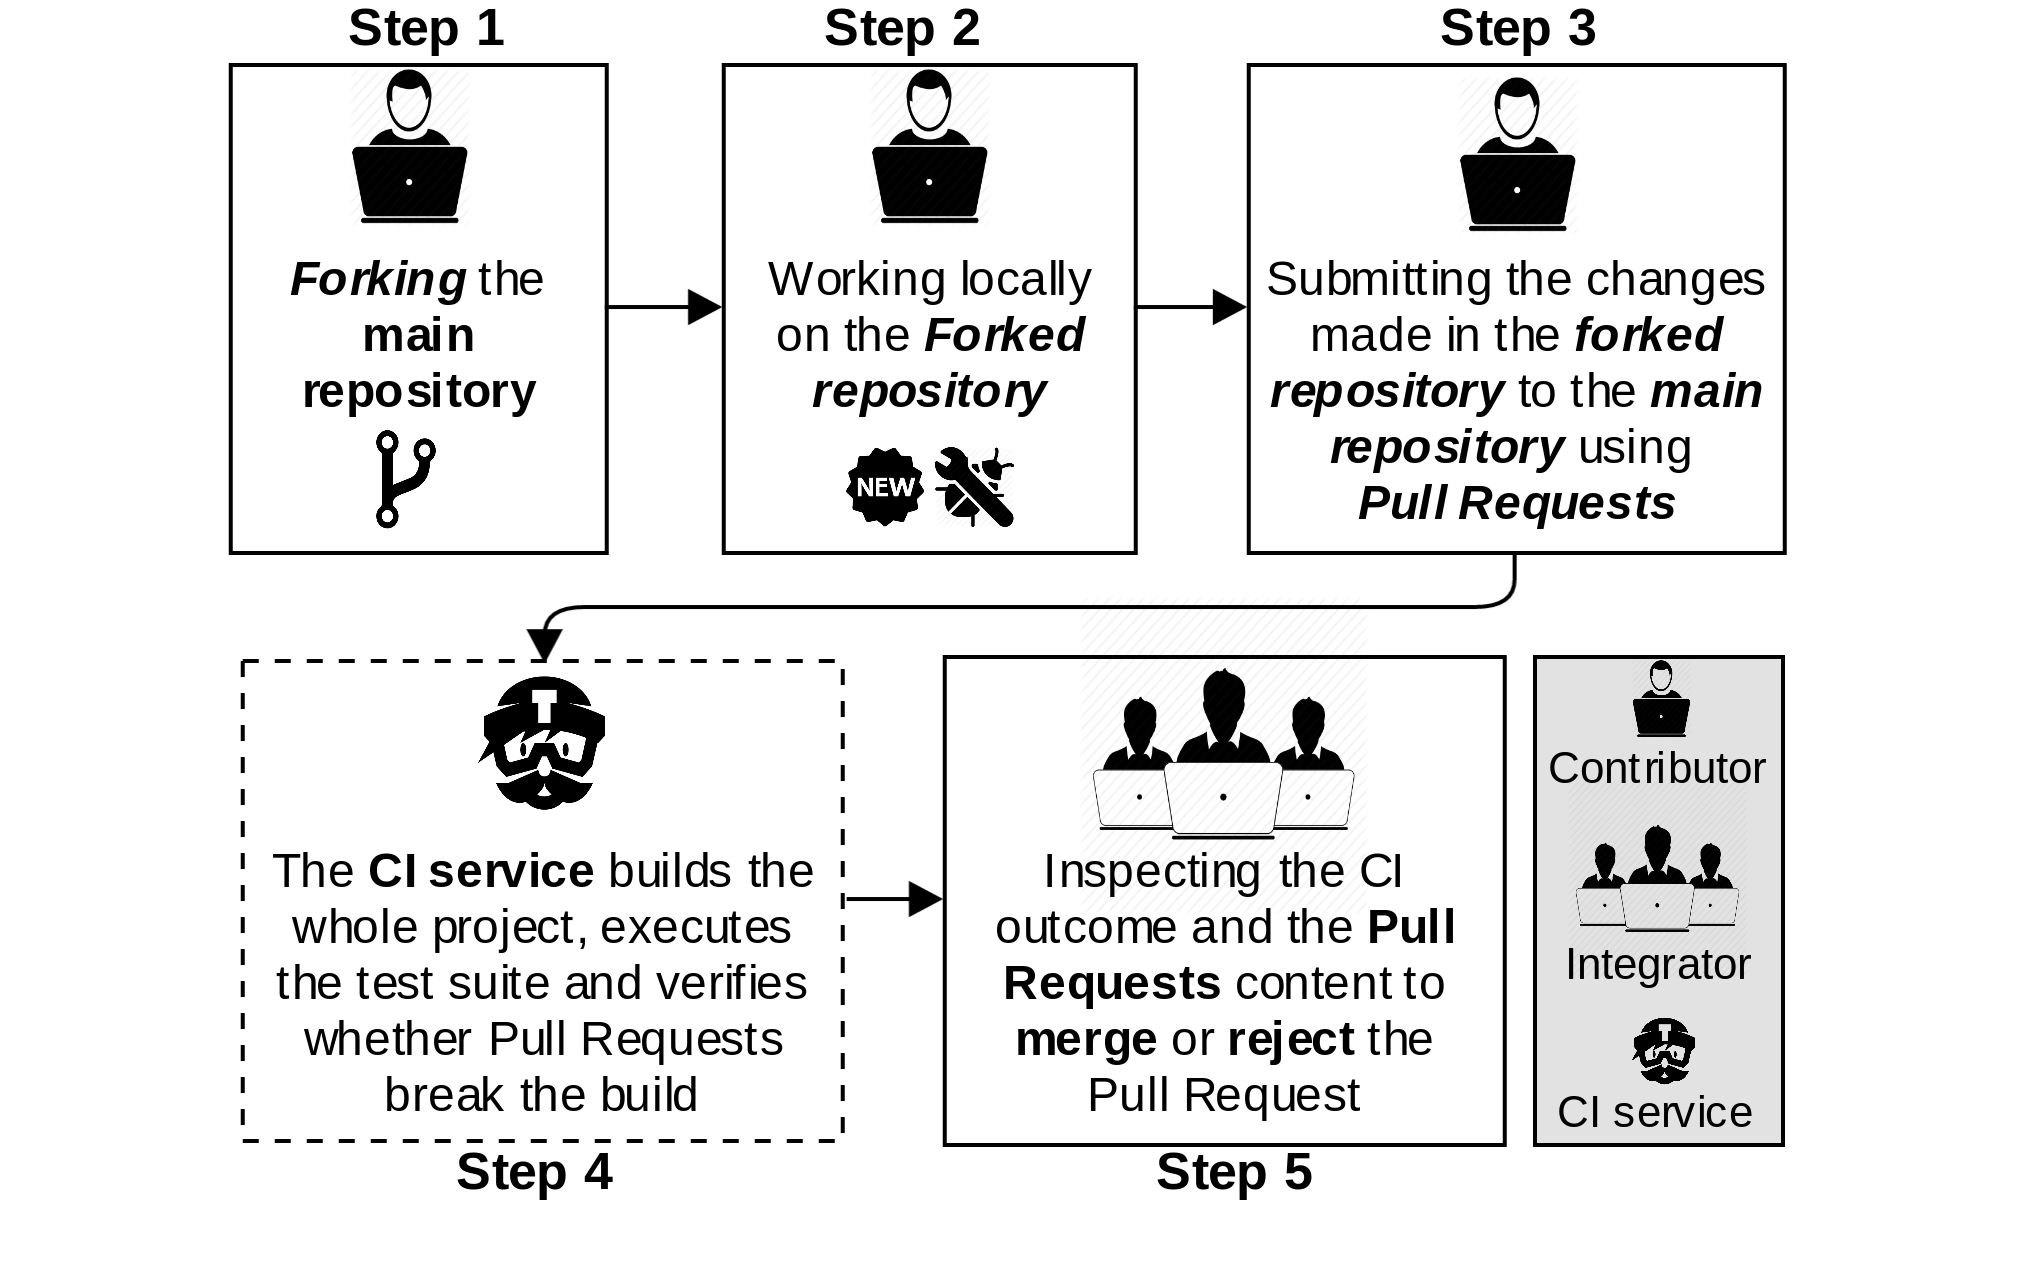
\includegraphics[width=3.5in]{img/pull-based-model.png}
	%\vspace{-2.3em}
	\caption{An overview of the pull-based development model that is
	integrated with Continuous Integration. The Step 4 is only performed when CI is used.}
	%\vspace{-1.5em}
	\label{fig:pull_based_development}
\end{figure}

{\em\textbf{Step 1. Fork a repository.}} The main repository of a project is not shared to external contributors. Instead, contributors can copy the main repository by forking it, so they can modify the code without interfering in other repositories and with no need of being a team member.

{\em\textbf{Step 2. Work locally in the forked repository.}} The contributors develop new functionalities, fix bugs or provide features and enhancements to the forked repository. 

{\em\textbf{Step 3. Submit the local changes to the main repository.}} When changes are ready to be submitted, contributors request a pull of such changes to the main repository by sending a pull request (PR) \citep{Yu2016-cy}. The PR specifies the local branch that has to be merged into a given branch of the main repository.

{\em\textbf{Step 4. Verify whether the PR breaks the build.}} The CI service automatically merges the PR into a test branch. Next, the CI service builds the whole project and runs the test suite to verify whether the PR breaks the codebase. Then, the build status becomes available to the contributor and integrators of the software project.

{\em\textbf{Step 5. Accept or reject a PR.}} 
After the PR submission, an integrator of the main repository must inspect the changes to decide whether they are satisfactory.  Typically, if tests fail during the process of CI (Step 4), the PR is rejected and additional changes are required by the external contributor to improve his/her PR \citep{Yu2016-cy}. In case all tests pass during the CI process, the integrators thoroughly review the PR before deciding whether to accept the contributions. This decision is based on the quality and technical design of the submitted PR as well as the priorities of the project.  In the pull-based development, the integrator plays a crucial role by managing contributions \citep{Gousios2015-ui}.

\subsection{\textbf{Continuous Integration in a pull-based development model}}
\label{subsec:pull_based_with_ci}

CI is a set of practices that allows developers to integrate their work more frequently, i.e., at least daily \citep{Fowler2006-zc,Meyer2014-px}. All code must be maintained in a single repository. When a contributor commits to the repository, an automated system verifies whether the change breaks the codebase (\textit{Step 4} of Figure \ref{fig:pull_based_development}) \citep{Meyer2014-px}. The entire process must be automated. Ideally, a build should compile the code and run a test suite to verify whether the codebase is broken after adding new changes. In CI, the work of developers is continually
compiled, built, and tested, following the philosophy that the system should always be in a working state~\citep{Yu2016-cy,Duvall2007-tb}

CI is widely used on GitHub. According to Gousios \textit{et al.} \citep{Gousios2015-ui}, 75\% of GitHub projects that make heavy use of PRs also tend to use CI. Several CI services, such as Jenkins, TeamCity, Bamboo, CloudBees and \texttt{Travis CI} \citep{Meyer2014-px} are available for development teams.  Jenkins and \texttt{Travis CI} are the most used by GitHub projects \citep{Vasilescu2015-tn}. \texttt{Travis CI} is a CI platform for open-source and private GitHub projects. Currently, over 300k projects are using this tool.

Beyond CI practice, Continuous Delivery (CDE) and Continuous Deployment (CD) are also complementary practices that can be used in the agile releasing engineering environment. CDE is a practice to automate the software delivery process of software projects, and it is often considered to extent CI \citep{Karvonen201787}. Therefore, in a project that uses CDE, the delivery can occur at any time, with little manual labor required. With CDE, the release schedule is in the hand of the business, whenever they want to make a release, the software should be ready to be released (what is assured by CI). Furthermore, the CD refers to a practice in which projects release each valid build triggered by a push or merged PR to users automatically. In summary, CI is a prerequisite for CDE, which is a prerequisite for CD.